\chapter{Tangkapan Layar Implementasi \textit{Hospital Client}}
\label{lampiran:implementasi-hospital-client}

Gambar~\ref{fig:halaman-dashboard-medical-personnel} sampai Gambar~\ref{fig:halaman-penulisan-segmen-rme-hospital-client} menampilkan antarmuka \textit{Hospital Client} hasil implementasi. Seluruh tangkapan layar merupakan dokumentasi penulis.

\begin{figure}[H]
	\centering
	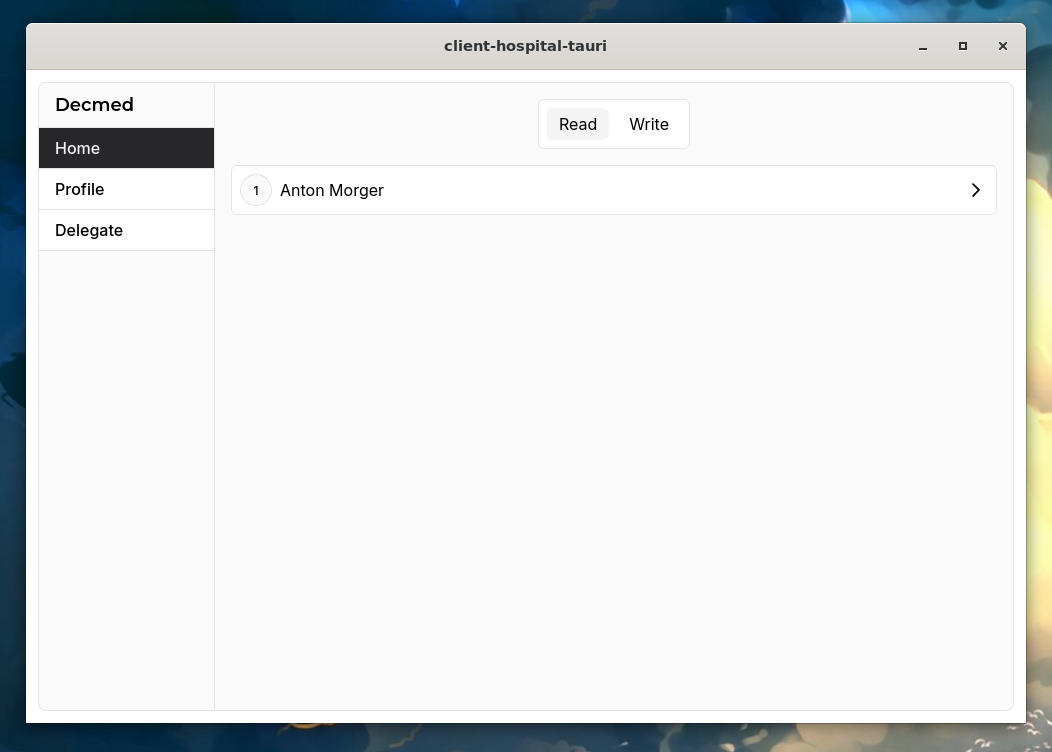
\includegraphics[width=0.85\textwidth]{resources/appendix/client/hospital/dashboard.png}
	\caption{Halaman \textit{dashboard} \textit{MedicalPersonnel}.}
	\label{fig:halaman-dashboard-medical-personnel}
\end{figure}

\begin{figure}[H]
	\centering
	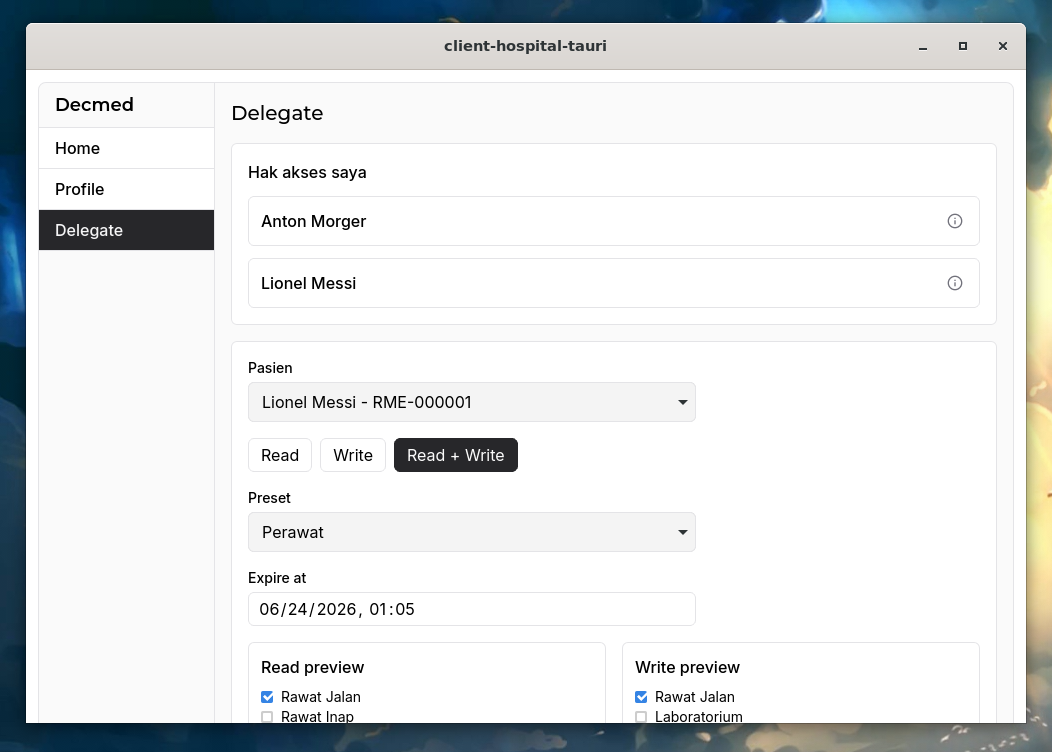
\includegraphics[width=0.85\textwidth]{resources/appendix/client/hospital/delegate 1.png}
	\caption{Halaman delegasi akses bagian 1.}
	\label{fig:halaman-delegasi-akses-bagian-1}
\end{figure}

\begin{figure}[H]
	\centering
	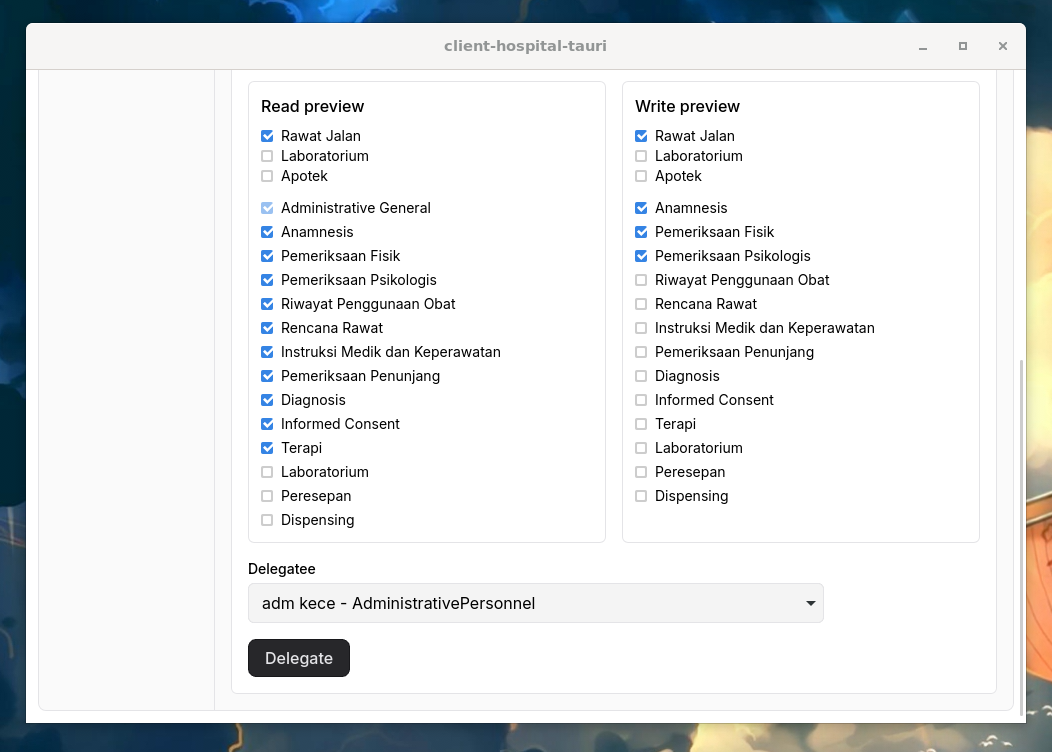
\includegraphics[width=0.95\textwidth]{resources/appendix/client/hospital/delegate 2.png}
	\caption{Halaman delegasi akses bagian 2.}
	\label{fig:halaman-delegasi-akses-bagian-2}
\end{figure}

\begin{figure}[H]
	\centering
	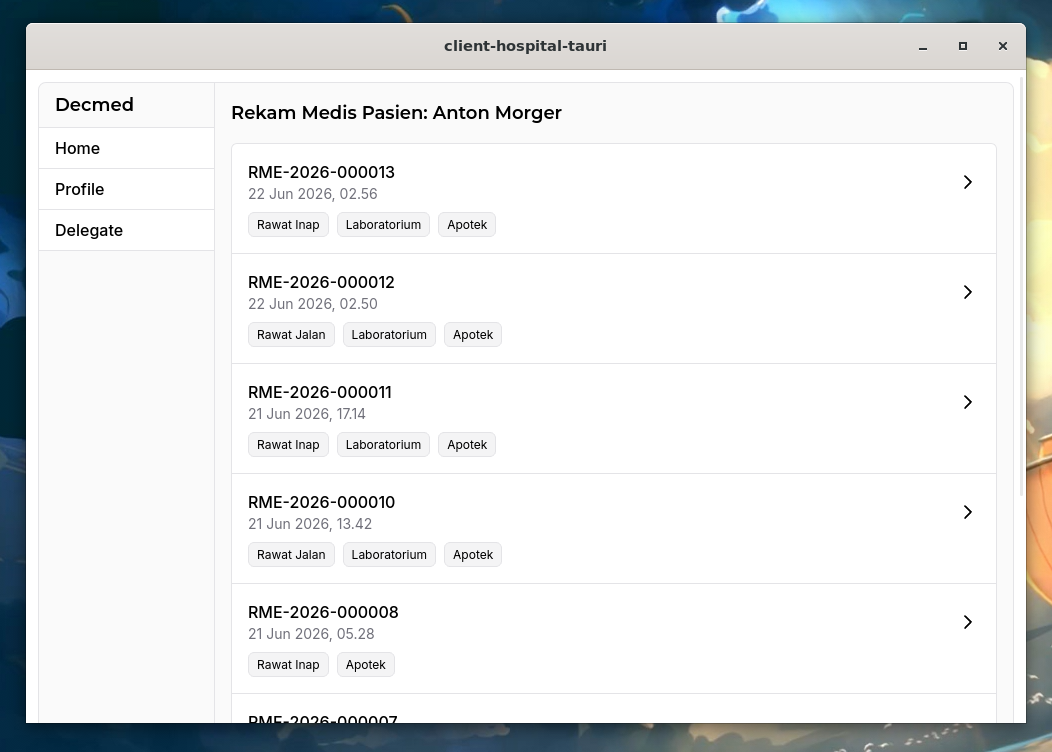
\includegraphics[width=0.95\textwidth]{resources/appendix/client/hospital/dashboard pasien.png}
	\caption{Halaman daftar RME pasien pada \textit{Hospital Client}.}
	\label{fig:halaman-daftar-rme-pasien-hospital-client}
\end{figure}

\begin{figure}[H]
	\centering
	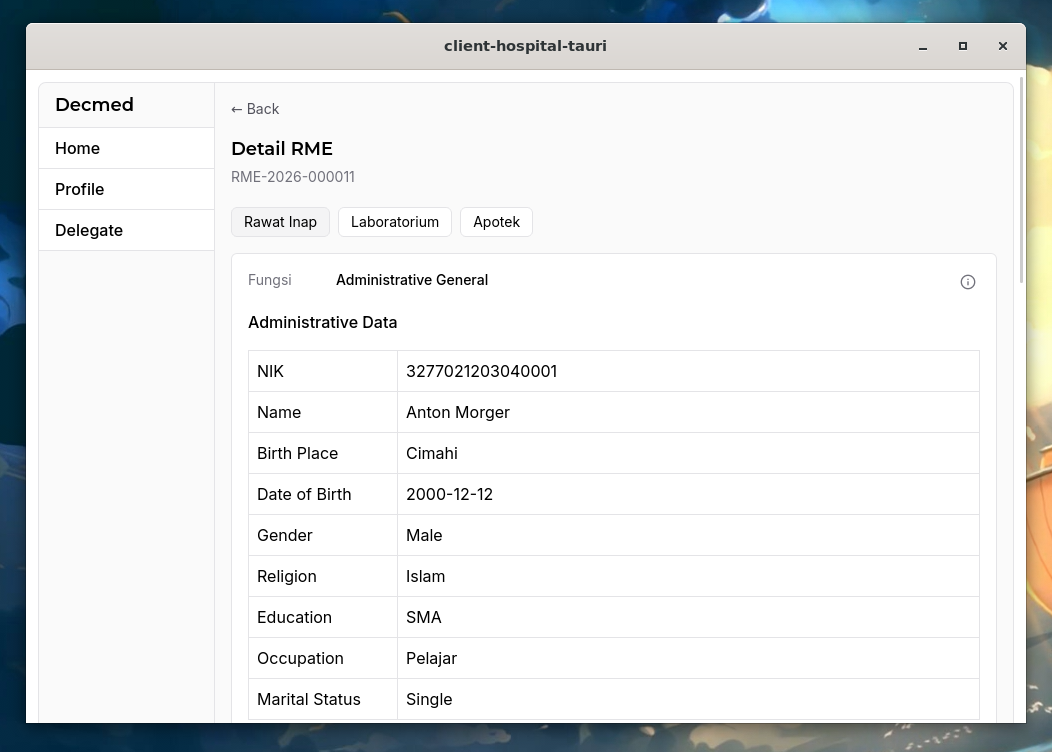
\includegraphics[width=0.95\textwidth]{resources/appendix/client/hospital/dashboard detail rme.png}
	\caption{Halaman detail RME pada \textit{Hospital Client}.}
	\label{fig:halaman-detail-rme-hospital-client}
\end{figure}

\begin{figure}[H]
	\centering
	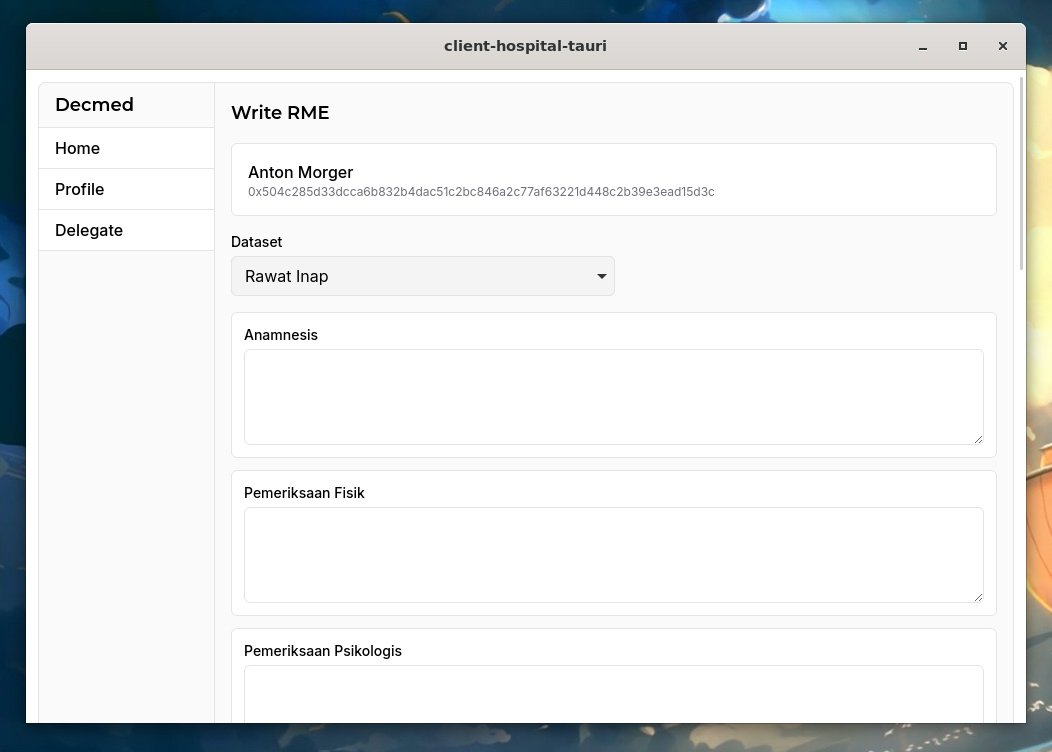
\includegraphics[width=0.95\textwidth]{resources/appendix/client/hospital/akses tulis.png}
	\caption{Halaman alur akses tulis pada \textit{Hospital Client}.}
	\label{fig:halaman-penulisan-segmen-rme-hospital-client}
\end{figure}